\section{Introduction}
In the original Bitcoin paper~\cite{bitcoin}, Nakamoto refers to
Bitcoin as a \emph{distributed timestamping server}.
% However, timestamps in adversarially produced blocks may be fabricated.
% And yet, empirical evidence suggests reported timestamps roughly correspond
% to real world time.
Chain timestamps have long been assumed to correspond to real-world time by the community.
DeFi applications with more than \$1B in monthly volume
rely~\cite{0x-timestamp} on the precision of these recorded timestamps.
They assume new transactions are not only
included soon --- a well-understood property known as \emph{liveness} ---
but also that their on-chain recorded timestamps are not far in the past compared to real time.
It is indeed the case that, in practical blockchain deployments, honest nodes only accept
blocks with timestamps up to a short window into the future\footnote{
  For example, this is part of the Bitcoin~\cite{bitcoin-code-future-blocks}
  and Ethereum~\cite{geth-future-blocks} implementations.
}.
% In community discussions, it has been incorrectly
% claimed
% \footnote{2016, Badr Bellaj, \href{https://ethereum.stackexchange.com/questions/6795/is-block-timestamp-safe-for-longer-time-periods}{\emph{Is block.timestamp safe for longer time periods?}}, Ethereum StackExchange.}
% that all accepted block timestamps must be within that same window of accuracy.
% \textcolor{red}{But this question asks about whether timestamps are accurate up to a month. That shouldn't be wrong, no? Could be removed.}
However, an adversary can produce a block with a fabricated past timestamp,
and can still cause this block to be accepted by the honest nodes retroactively by, for example, cooking
up a lucky slightly longer Bitcoin chain. In this paper, we show that these fabrications
cannot exceed a certain \emph{timeliness} limit, which we calculate.


We put forth the notion of \emph{timeliness}, formalizing the folklore
understanding that timestamps recorded on-chain cannot deviate arbitrarily
from real world time. In particular, we define a timeliness parameter $v$ which bounds
how far in the past a timestamp can be. Under a synchronous network, a global clock, and honest majority, we prove this virtue materializes in all three popular flavors of
permissionless blockchains, namely proof-of-work,
longest chain proof-of-stake, and quorum-based proof-of-stake, and analytically
calculate their timeliness parameter.

Blockchain systems executed in networks with delay, even when assuming a global clock and
bounded delay, allow honest parties to reach consensus, but the ledgers reported by
honest parties are typically merely prefixes of one another.
Under perfectly synchronized clocks, we show that any \emph{timely} blockchain can be modified to achieve
\emph{exactly equal} ledgers at every point in time, a property we call \emph{supersafety},
albeit with the introduction of a small confirmation delay.

The introduction of these two
properties in this abstract fashion simplifies the proofs of security of protocols built on
top. For example, cross-chain constructions such as Babylon~\cite{babylon} are simpler
to prove if on-chain timestamps are used instead of block heights,
but timeliness is needed to do this.
Consensus constructions which require the synchronized production of randomness,
such as Ouroboros~\cite{ouroboros,praos}, can also benefit by simpler security
arguments from the abstraction of the supersafety property.

\noindent
\textbf{Our contributions.} In this paper, we make the following contributions:

\begin{enumerate}
  \item We introduce the notion of ledger \emph{timeliness}.
        We prove that three exemplary cases of blockchain protocols (Bitcoin, Streamlet, and Ouroboros)
        are timely and calculate their timeliness(Section~\ref{sec:possible}). We also show that network synchrony is required for timeliness (Section~\ref{sec:impossibility}).
  \item We build a \emph{supersafe} protocol from any timely ledger.
        Supersafe protocols allow parties with synchronized clocks to
        reach the exact same conclusion about their ledgers at the exact same time.
        Conversely, we reduce from supersafety back to timeliness, illustrating that
        the two properties are morally equivalent.
\end{enumerate}

\begin{figure}
  \centering
  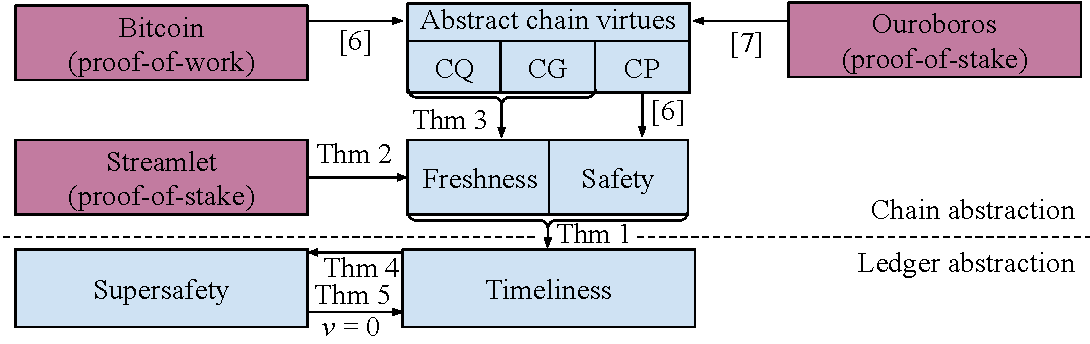
\includegraphics[width=1.0\columnwidth,keepaspectratio]{figures/timeliness-overview.pdf}
  \caption{Paper overview. Bitcoin and Ouroboros attain the abstract chain virtues
  of Common Prefix, Chain Quality, and Chain Growth (top)~\cite{backbone,ouroboros}.
  We show that CQ and CG imply the intermediate property of freshness
  (Theorem~\ref{thm:longest-chain-freshness}, middle). This property is also achieved by Streamlet
  (Theorem~\ref{thm:streamlet-freshness}), which is different from the other two longest-chain protocols. This property, together with safety,
  is sufficient to prove timeliness
  (Theorem~\ref{thm:freshness-to-timeliness}). In safe and live protocols, from timeliness we can achieve supersafety
  and vice versa (Theorems~\ref{thm:timeliness-to-supersafety}-\ref{thm:backward-reduction}, bottom).
  \textcolor{red}{Broken references. What should these point to?}
  }
 \label{fig:overview}
\end{figure}

\noindent
\textbf{Overview of the results.}
An overview of the results of this paper is illustrated in Figure~\ref{fig:overview}.
Our first result is proving that all popular ways of constructing distributed ledgers
are, indeed, timely, if we assume a global clock and a synchronous network.
The timeliness follows from an intermediate technical property we call \emph{freshness}
of chains, which we prove for three protocols
Streamlet, Bitcoin Backbone, and Ouroboros, that are representatives
of the three major classes of protocols: quorum-based proof-of-stake, longest chain
proof-of-work, and longest chain proof-of-stake respectively (Section~\ref{sec:possible}).
The Streamlet variant is proven in the partially synchronous setting after GST.
We show that timeliness before GST is impossible for protocols that are always-safe
and live after GST (Section~\ref{sec:impossibility}).
In practice, the assumption of a global clock can be relaxed by tolerating an additional deviation in the timestamps equal to the maximum clock deviation.

Next, we perform two simple but instructive black-box reductions that are, perhaps, somewhat unexpected:
The first reduction is from timeliness to supersafety (Section~\ref{sec:forward-reduction}).
In this reduction, we delay the reported ledger until all
transactions have timestamps enough into the past to ensure all other parties have seen them.
This allows us to achieve a remarkable property: All honest parties report the
exact same ledgers at the exact same time.
In this reduction, parties who desire supersafety for their application can individually choose to obtain supersafety at the cost of additional confirmation delay, while other parties continue to have faster confirmation and standard safety. 
The second reduction is from supersafety back to (perfect) timeliness (Section~\ref{sec:backward-reduction}).
To do this, every online node reports the new transactions they see with
their current timestamp, and due to supersafety, these are the same.
Some additional work is needed to allow intermittently online nodes to catch up, which we also show.

\noindent
\textbf{Related work.}
Arguments of chain timeliness appear at the heart of various security proofs
in the blockchain literature.
In the variable difficulty Bitcoin Backbone paper~\cite{varbackbone},
it is shown that the different honest parties performing target recalculation on different chains
must arrive at roughly the same result, relying on roughly synchronized timestamps.
In the Ouroboros protocol~\cite{ouroboros},
the randomness production from epoch-to-epoch requires chopping off a suitable number of \emph{slots},
achieving a form of supersafety. The blockchain itself has also been used~\cite{klepsydra,chronos}
as a mechanism for clock synchronization among parties with desynchronized and drifting clocks,
a long-standing problem~\cite{lamport-synchronizing-clocks}.
In our work, we show that, if the clocks of honest parties are already synchronized,
on-chain reported timestamps roughly correspond to real-world time.
\textcolor{red}{Logical clocks versus real-world time? How are their techniques related to ours and could they be used to derive timeliness or any additional properties?}
We posit that the abstraction of timeliness and supersafety
into stand-alone properties can aid in simplifying the security proofs
of existing and future protocols.
\textcolor{red}{TODO: Comparison and reference to GearBox.}

Previously, the community was confused about whether on-chain timestamps are accurate.
In some discussions, it was incorrectly
claimed\footnote{2016, Badr Bellaj, \href{https://ethereum.stackexchange.com/a/9752}{\emph{Is block.timestamp safe for longer time periods?}}, Ethereum StackExchange.} that all accepted block timestamps must be within the same tolerance that honest nodes use to accept blocks, ignoring the possibility of fabricated timestamps in blocks produced by the adversary.
On the other hand, others conjectured that on-chain timestamps can be vastly
inaccurate stating that \emph{timestamps can differ radically from the
actual time, outside the network}~\cite{szalachowski2018short}.
In this work, we resolve this confusion, derive the timeliness parameter and rigorously show the conditions under which it holds.
% In this work, we debunk this misconception, and rigorously show that the chain itself
% guarantees a modest level of timeliness internally.
Supersafety, although never stated formally, was achieved since the early
days of consensus by Dolev and Strong~\cite{dolev-strong}.
However, contrary to us, their construction does not support intermittently online (sleepy) clients,
and was designed for a different era of consensus, with a much smaller scale
than today's systems in mind, poor performance, and no support for dynamic availability.
